\section{Auswertung}
Zuerst wird die Schaltung aus \autoref{fig:3} in der \autoref{sec:Theorie} aufgebaut und wie in der \autoref{sec:Theorie} beschrieben
Die Spannungsamplitude in abhängigkeit der Phase betrachtet.
\begin{table}[H]
    \centering
    \caption{}
    \label{tab:t2}
    \begin{tblr}{
        colspec = {S S },
        row{1} = {guard, mode=math},}
           \toprule
            \text{Phase} \left(\unit{\degree}\right) & U \left(\unit{\volt}\right)\\
           \midrule
            30  &3\\
            60  &6\\
            90  &6\\
            120 &5.5\\
            150 &2\\
            180 &-0.5\\
            210 &-3\\
            240 &-5.5\\
            270 &-6\\
            300 &-5.5\\
            330 &-2\\
            630 &0\\
            \bottomrule
    \end{tblr}
\end{table}

%Plot Phase/Spannung
\begin{figure}[H]
    \caption{}
    \label{fig:10}
    \centering
    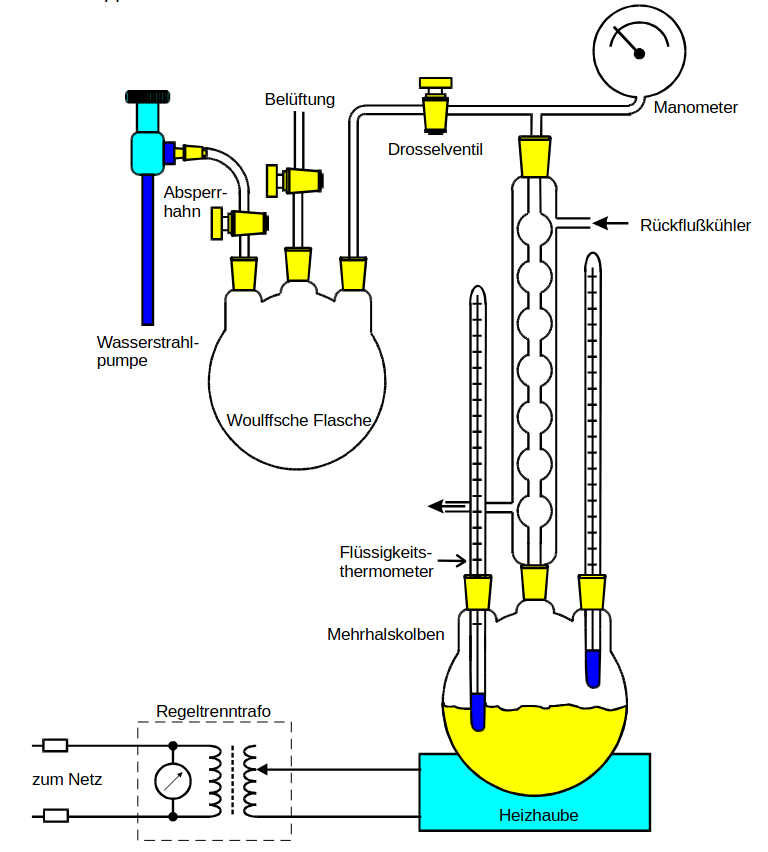
\includegraphics{"build/teil1.pdf"}
\end{figure}


%Intensität/Abstand
\begin{figure}[H]
    \caption{}
    \label{fig:10}
    \centering
    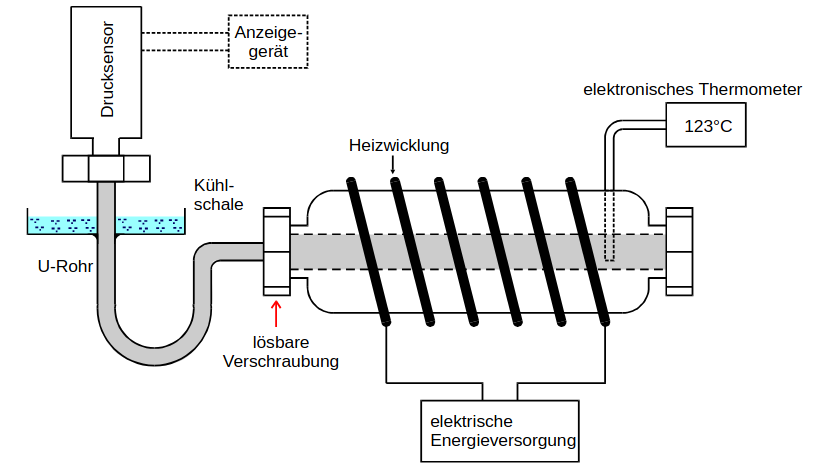
\includegraphics{"build/teil2.pdf"}
\end{figure}

\label{sec:Auswertung}
